\subsection{DATA SHEET \#2}
	\begin{enumerate}[A.]
		\item Circuit \#1: Direct measurement of potential changes (voltage) using the DMM across each resistor separately and both together.  Assume uncertainty of 0.05\%.\\
		
			$\Delta V_1 \pm uncertainty = 5.344 \pm 0.0027 V$\\
			$\Delta V_2 \pm uncertainty = 3.1904 \pm 0.0016 V$\\
			$\Delta V_{TOTAL} \pm uncertainty = 8.533 \pm 0.0043 V$\\
			
		\item Compare the values of voltages calculated in C1 (DATA SHEET \#1 with those directly measured in Part D above.  Do this by plotting the values appropriately on the grid below, setting the vertical scale so the uncertainty bars on the values are visible.  No horizontal axis scale is needed.  Simply plot the points next to each other.  For example, do the uncertainty ranges of $\Delta V_{1CALC} \pm uncertainty$ and $\Delta V_{1} \pm uncertainty$ overlap?\\
		
		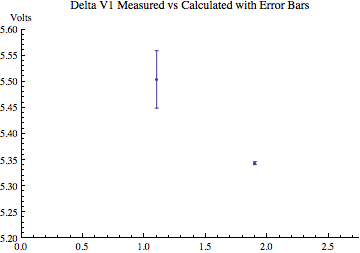
\includegraphics[width=200px]{lab6_graph1_deltav1}
		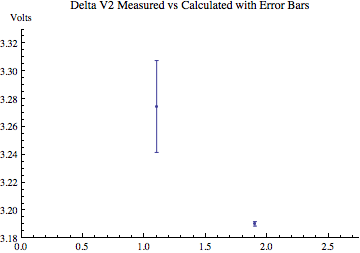
\includegraphics[width=200px]{lab6_graph2_deltav2}
		
		\item Comment on the above results.  Are the measurements consistent with each other? \\
		
		Within the given uncertainty terms, no they are not consistent with one another in the sense that the two sets of intervals do not overlap.  They do, however, appear to be correlated within a lower confidence interval.
\end{enumerate}
		